\documentclass[12pt]{article}
\usepackage[paperwidth=25cm,paperheight=17cm,margin=1.4cm]{geometry}
\usepackage[T1]{fontenc}
\usepackage[utf8]{inputenc}
\usepackage[magyar]{babel}
\usepackage{lmodern}
\usepackage{amsmath,amssymb}
\usepackage{enumitem}
\usepackage{array}
\usepackage{tikz}
\usetikzlibrary{arrows.meta,patterns,calc}
\usepackage[most]{tcolorbox}

\pagestyle{empty}
\setlength{\parindent}{0pt}
\setlength{\parskip}{4pt}
\setlist[itemize]{leftmargin=1.4em, itemsep=3pt, topsep=2pt, parsep=0pt}

\newcommand{\dia}[1]{\newpage{\Large\bfseries #1}\par\vspace{2pt}{\color{blue!50!black}\hrule height 1pt}\vspace{8pt}}

\newtcolorbox{pelda}[1][]{colback=green!4,colframe=green!45!black,fonttitle=\bfseries,
  title=Kidolgozott példa,left=5pt,right=5pt,top=3pt,bottom=3pt,before skip=6pt,after skip=4pt,#1}
\newtcolorbox{fontos}[1][]{colback=blue!3,colframe=blue!45!black,
  left=5pt,right=5pt,top=3pt,bottom=3pt,before skip=6pt,after skip=4pt,#1}

% Lencsés képszerkesztés: #1 = f, #2 = t, #3 = tárgymagasság, #4 = xmin, #5 = xmax
\newcommand{\lenskep}[5]{%
  \pgfmathsetmacro{\kk}{1/(1/#1 - 1/#2)}%
  \pgfmathsetmacro{\KK}{-#3*\kk/#2}%
  \pgfmathsetmacro{\HH}{max(#3,abs(\KK))+0.45}%
  \pgfmathtruncatemacro{\virt}{\kk<0 ? 1 : 0}%
  \pgfmathtruncatemacro{\gyujto}{#1>0 ? 1 : 0}%
  \draw[->,gray] (#4,0) -- (#5,0);
  \ifnum\gyujto=1
    \draw[{Stealth[length=2mm]}-{Stealth[length=2mm]},thick,blue!60!black] (0,-\HH) -- (0,\HH);
  \else
    \draw[{Stealth[length=2mm,reversed]}-{Stealth[length=2mm,reversed]},thick,blue!60!black] (0,-\HH) -- (0,\HH);
  \fi
  \fill (#1,0) circle (1.5pt) node[below,font=\scriptsize] {$F$};
  \fill (-#1,0) circle (1.5pt) node[below,font=\scriptsize] {$F$};
  \draw[very thick,-{Stealth[length=2mm]}] (-#2,0) -- (-#2,#3);
  \begin{scope}
    \clip (#4,-\HH-0.3) rectangle (#5,\HH+0.3);
    \ifnum\gyujto=1
      \draw[red!75!black] (-#2,#3) -- (0,#3) -- ($(0,#3)!8!(#1,0)$);
    \else
      \draw[red!75!black] (-#2,#3) -- (0,#3) -- ($(0,#3)!-8!(#1,0)$);
    \fi
    \draw[orange!85!black] (-#2,#3) -- ($(-#2,#3)!8!(0,0)$);
    \ifnum\virt=1
      \draw[red!75!black,dashed] (0,#3) -- (\kk,\KK);
      \draw[orange!85!black,dashed] (0,0) -- (\kk,\KK);
      \ifnum\gyujto=0 \draw[red!75!black,dashed] (\kk,\KK) -- (#1,0); \fi
      \draw[very thick,dashed,green!50!black,-{Stealth[length=2mm]}] (\kk,0) -- (\kk,\KK);
    \else
      \draw[violet] (-#2,#3) -- (0,\KK) -- (#5,\KK);
      \draw[very thick,green!50!black,-{Stealth[length=2mm]}] (\kk,0) -- (\kk,\KK);
    \fi
  \end{scope}
}

% Képszerkesztés lencsével (melléklet): #1 = f, #2 = t, #3 = T, #4 = xmin, #5 = xmax
\newcommand{\Lkep}[5]{%
  \pgfmathtruncatemacro{\Lvegt}{abs(#2-#1)<0.01 ? 1 : 0}%
  \ifnum\Lvegt=0
    \pgfmathsetmacro{\Lk}{1/(1/#1 - 1/#2)}%
    \pgfmathsetmacro{\LK}{-#3*\Lk/#2}%
    \pgfmathtruncatemacro{\Lvirt}{\Lk<0 ? 1 : 0}%
  \else \def\Lvirt{2}\fi
  \pgfmathtruncatemacro{\Lgy}{#1>0 ? 1 : 0}%
  \useasboundingbox (#4,-2.1) rectangle (#5,2.1);
  \draw[->,gray] (#4,0) -- (#5,0);
  \ifnum\Lgy=1
    \draw[{Stealth[length=2mm]}-{Stealth[length=2mm]},thick,blue!60!black] (0,-1.85) -- (0,1.85);
  \else
    \draw[{Stealth[length=2mm,reversed]}-{Stealth[length=2mm,reversed]},thick,blue!60!black] (0,-1.85) -- (0,1.85);
  \fi
  \foreach \s in {1,-1} {\fill (\s*#1,0) circle (1.5pt); \draw (\s*2*#1,-0.08) -- (\s*2*#1,0.08);}
  \node[below left,font=\scriptsize,inner sep=1.5pt] at (-#1,0) {$F$};
  \node[below right,font=\scriptsize,inner sep=1.5pt] at (#1,0) {$F$};
  \node[below left,font=\scriptsize,inner sep=1.5pt] at (-2*#1,0) {$2F$};
  \node[below right,font=\scriptsize,inner sep=1.5pt] at (2*#1,0) {$2F$};
  \draw[very thick,-{Stealth[length=2mm]}] (-#2,0) -- (-#2,#3);
  \begin{scope}
    \clip (#4,-2.1) rectangle (#5,2.1);
    \ifnum\Lgy=1
      \draw[semithick,red!75!black] (-#2,#3) -- (0,#3) -- ($(0,#3)!10!(#1,0)$);
    \else
      \draw[semithick,red!75!black] (-#2,#3) -- (0,#3) -- ($(0,#3)!-10!(#1,0)$);
    \fi
    \draw[semithick,orange!85!black] (-#2,#3) -- ($(-#2,#3)!10!(0,0)$);
    \ifcase\Lvirt
      \draw[semithick,violet] (-#2,#3) -- (0,\LK) -- (#5,\LK);
      \draw[very thick,green!50!black,-{Stealth[length=2mm]}] (\Lk,0) -- (\Lk,\LK);
    \or
      \ifnum\Lgy=1
        \draw[semithick,red!75!black,dashed] (0,#3) -- (\Lk,\LK);
        \draw[semithick,orange!85!black,dashed] (-#2,#3) -- (\Lk,\LK);
      \else
        \draw[semithick,red!75!black,dashed] (0,#3) -- (#1,0);
      \fi
      \draw[very thick,dashed,green!50!black,-{Stealth[length=2mm]}] (\Lk,0) -- (\Lk,\LK);
    \fi
  \end{scope}
}

% Képszerkesztés gömbtükörrel (melléklet): #1 = f, #2 = t, #3 = T, #4 = xmin, #5 = xmax
% A tükör a tengelyt az origóban metszi, a fény balról jön. Homorú: f > 0, domború: f < 0.
\newcommand{\Tkep}[5]{%
  \pgfmathsetmacro{\Tsg}{#1>0 ? -1 : 1}%
  \pgfmathtruncatemacro{\Tvegt}{abs(#2-#1)<0.01 ? 1 : 0}%
  \pgfmathsetmacro{\Txa}{\Tsg*0.15*#3*#3/3.4225}%
  \ifnum\Tvegt=0
    \pgfmathsetmacro{\Tk}{1/(1/#1 - 1/#2)}%
    \pgfmathsetmacro{\TK}{-#3*\Tk/#2}%
    \pgfmathsetmacro{\Tix}{-\Tk}%
    \pgfmathsetmacro{\Txb}{\Tsg*0.15*\TK*\TK/3.4225}%
    \pgfmathtruncatemacro{\Tvirt}{\Tk<0 ? 1 : 0}%
  \else \def\Tvirt{2}\fi
  \useasboundingbox (#4,-2.1) rectangle (#5,2.1);
  \draw[->,gray] (#4,0) -- (#5,0);
  \draw[very thick,blue!60!black,domain=-1.85:1.85,samples=31,smooth,variable=\y]
    plot ({\Tsg*0.15*\y*\y/3.4225},\y);
  \foreach \y in {-1.75,-1.45,...,1.9}
    \draw[blue!60!black] ({\Tsg*0.15*\y*\y/3.4225},\y) -- ++(0.18,0.14);
  \fill (-#1,0) circle (1.5pt); \fill (-2*#1,0) circle (1.5pt);
  \pgfmathtruncatemacro{\Thom}{#1>0 ? 1 : 0}%
  \ifnum\Thom=1
    \node[below left,font=\scriptsize,inner sep=1.5pt] at (-#1,0) {$F$};
    \node[below left,font=\scriptsize,inner sep=1.5pt] at (-2*#1,0) {$C$};
  \else
    \node[below right,font=\scriptsize,inner sep=1.5pt] at (-#1,0) {$F$};
    \node[below right,font=\scriptsize,inner sep=1.5pt] at (-2*#1,0) {$C$};
  \fi
  \draw[very thick,-{Stealth[length=2mm]}] (-#2,0) -- (-#2,#3);
  \begin{scope}
    \clip (#4,-2.1) rectangle (#5,2.1);
    \draw[semithick,red!75!black] (-#2,#3) -- (\Txa,#3);
    \draw[semithick,orange!85!black] (-#2,#3) -- (0,0) -- ($(0,0)!10!(-#2,-#3)$);
    \ifcase\Tvirt
      \draw[semithick,red!75!black] (\Txa,#3) -- ($(\Txa,#3)!10!(\Tix,\TK)$);
      \draw[semithick,violet] (-#2,#3) -- (\Txb,\TK) -- (#4,\TK);
      \draw[very thick,green!50!black,-{Stealth[length=2mm]}] (\Tix,0) -- (\Tix,\TK);
    \or
      \draw[semithick,red!75!black] (\Txa,#3) -- ($(\Txa,#3)!-10!(\Tix,\TK)$);
      \ifnum\Thom=1
        \draw[semithick,red!75!black,dashed] (\Txa,#3) -- (\Tix,\TK);
      \else
        \draw[semithick,red!75!black,dashed] (\Txa,#3) -- (-#1,0);
      \fi
      \draw[semithick,orange!85!black,dashed] (0,0) -- (\Tix,\TK);
      \draw[very thick,dashed,green!50!black,-{Stealth[length=2mm]}] (\Tix,0) -- (\Tix,\TK);
    \or
      \draw[semithick,red!75!black] (\Txa,#3) -- ($(\Txa,#3)!10!(-#1,0)$);
    \fi
  \end{scope}
}

% egy cella a mellékletben: #1 = rajz, #2 = felirat
\newcommand{\cella}[2]{%
  \begin{minipage}[t]{0.32\linewidth}\centering
  \begin{tikzpicture}[x=0.95cm,y=0.95cm,>=Stealth]#1\end{tikzpicture}\\[4pt]
  \parbox{\linewidth}{\centering\small #2}
  \end{minipage}}

% jelmagyarázat-vonal
\newcommand{\jel}[1]{\tikz[baseline=-0.6ex]\draw[very thick,#1] (0,0) -- (0.6,0);}

\begin{document}

%====================================================================
\begin{center}
  \vspace*{1.2cm}
  {\Huge\bfseries Geometriai optika}\\[0.6cm]
  {\Large fénytörés, teljes visszaverődés, leképezés}\\[1.2cm]
\end{center}

\begin{center}
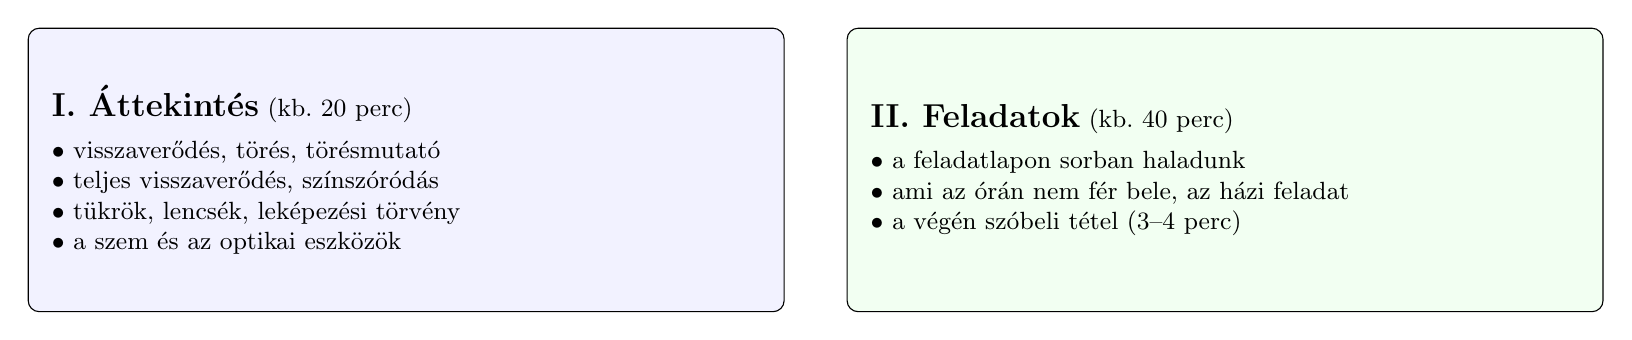
\begin{tikzpicture}[font=\small,
    resz/.style={draw,rounded corners,minimum width=9.6cm,minimum height=3.6cm,align=left,anchor=north}]
  \node[resz,fill=blue!5] at (-5.2,0) {%
    \parbox{9cm}{\textbf{\large I.\ Áttekintés} (kb.\ 20 perc)\\[4pt]
    $\bullet$ visszaverődés, törés, törésmutató\\
    $\bullet$ teljes visszaverődés, színszóródás\\
    $\bullet$ tükrök, lencsék, leképezési törvény\\
    $\bullet$ a szem és az optikai eszközök}};
  \node[resz,fill=green!5] at (5.2,0) {%
    \parbox{9cm}{\textbf{\large II.\ Feladatok} (kb.\ 40 perc)\\[4pt]
    $\bullet$ a feladatlapon sorban haladunk\\
    $\bullet$ ami az órán nem fér bele, az házi feladat\\
    $\bullet$ a végén szóbeli tétel (3--4 perc)}};
\end{tikzpicture}
\end{center}

\vspace{0.8cm}
\begin{center}
\small A fény elektromágneses hullám (6.\ óra), a törés ugyanaz a jelenség, mint a vízhullámoknál
(8.\ óra). Ha a fény útjába eső tárgyak sokkal nagyobbak a hullámhossznál, az elhajlás
elhanyagolható, és a fényt \textbf{egyenes sugarakkal} írhatjuk le: ez a geometriai optika.
\end{center}

%====================================================================
\dia{1. Visszaverődés és törés}

\begin{minipage}[t]{0.58\linewidth}\vspace{0pt}
\begin{itemize}
  \item Homogén közegben a fény egyenes vonalban terjed. Két közeg határán egy része
    \textbf{visszaverődik}, más része \textbf{megtörik}.
  \item \textbf{Visszaverődés:} a beesési szög egyenlő a visszaverődési szöggel
    ($\alpha = \alpha'$), a szögeket a beesési merőlegestől mérjük.
  \item \textbf{Abszolút törésmutató:} $n = \dfrac{c}{c_\text{közeg}}$ \;
    (vákuum: $1$, levegő: $\approx 1$, víz: $1{,}33$, üveg: $\approx 1{,}5$, gyémánt: $2{,}42$).
    A nagyobb törésmutatójú közeg \textbf{optikailag sűrűbb}: ott lassabb a fény.
\end{itemize}
\begin{fontos}
\centering \textbf{Snellius--Descartes-törvény:} \quad
$\dfrac{\sin\alpha}{\sin\beta} = \dfrac{c_1}{c_2} = \dfrac{n_2}{n_1} = n_{2,1}$
\quad (relatív törésmutató)\\[3pt]
Sűrűbb közegbe lépve a fény a merőlegeshez \textbf{törik}. A frekvencia (a szín) nem
változik, a hullámhossz igen: $\lambda_\text{közeg} = \lambda_0 / n$.
\end{fontos}
\begin{pelda}
Fény levegőből $\alpha = 30^\circ$-ban üvegre ($n = 1{,}5$) esik:
$\sin\beta = \tfrac{\sin 30^\circ}{1{,}5} = 0{,}333$ $\Rightarrow$ $\beta \approx 19{,}5^\circ$.
A fény sebessége az üvegben $c/n = 2\cdot 10^8~\tfrac{\text{m}}{\text{s}}$, a $600$~nm-es
fény hullámhossza ott $400$~nm.
\end{pelda}
\end{minipage}\hfill
\begin{minipage}[t]{0.38\linewidth}\vspace{0pt}\centering
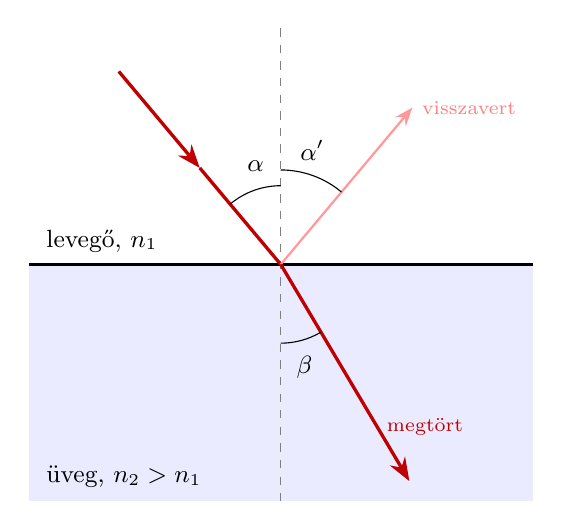
\begin{tikzpicture}[>=Stealth,font=\small]
  \fill[blue!8] (-3.2,-3) rectangle (3.2,0);
  \draw[thick] (-3.2,0) -- (3.2,0);
  \node[anchor=west] at (-3.1,0.3) {levegő, $n_1$};
  \node[anchor=west] at (-3.1,-2.7) {üveg, $n_2 > n_1$};
  \draw[dashed,gray] (0,3) -- (0,-3);
  \draw[very thick,red!75!black,->] (130:3.2) -- (130:1.6);
  \draw[very thick,red!75!black] (130:1.6) -- (0,0);
  \draw[thick,red!40,->] (0,0) -- (50:2.6);
  \draw[very thick,red!75!black,->] (0,0) -- (-59.3:3.2);
  \draw (0,1.0) arc (90:130:1.0); \node at (-0.32,1.25) {$\alpha$};
  \draw (0,1.2) arc (90:50:1.2); \node at (0.4,1.45) {$\alpha'$};
  \draw (0,-1.0) arc (-90:-59.3:1.0); \node at (0.3,-1.3) {$\beta$};
  \node[red!50,font=\scriptsize,anchor=west] at (50:2.6) {visszavert};
  \node[red!75!black,font=\scriptsize,anchor=west] at (-59.3:2.4) {megtört};
\end{tikzpicture}
\end{minipage}

%====================================================================
\dia{2. Teljes visszaverődés és színszóródás}

\begin{minipage}[t]{0.56\linewidth}\vspace{0pt}
\begin{itemize}
  \item Ha a fény optikailag \textbf{sűrűbb} közegből \textbf{ritkább} felé halad, a
    merőlegestől törik: $\beta > \alpha$. Annál a beesési szögnél, ahol $\beta = 90^\circ$
    lenne, a megtört sugár éppen a határfelület mentén halad: ez a \textbf{határszög}.
  \item Ennél nagyobb beesési szögnél nincs megtört sugár, a fény \textbf{teljes egészében
    visszaverődik}. (Sík tükörnél mindig van veszteség, itt nincs!)
\end{itemize}
\begin{fontos}
\[ \sin\alpha_\text{h} = \frac{n_2}{n_1} \qquad\text{(levegőbe kilépve: } \sin\alpha_\text{h} = \tfrac1n\text{)} \]
\centering Alkalmazás: \textbf{optikai szál} (internet, endoszkóp), prizmás távcső, a gyémánt csillogása.
\end{fontos}
\begin{itemize}
  \item \textbf{Színszóródás (diszperzió):} a törésmutató kicsit függ a színtől: az
    \textbf{ibolya} fény törik a legjobban, a \textbf{vörös} a legkevésbé. Ezért bontja a
    prizma színekre a fehér fényt, és ezért van szivárvány.
\end{itemize}
\begin{pelda}
Üveg--levegő határon: $\sin\alpha_\text{h} = \tfrac{1}{1{,}5}$ $\Rightarrow$
$\alpha_\text{h} \approx 41{,}8^\circ$. Gyémántnál $\sin\alpha_\text{h} = \tfrac{1}{2{,}42}$
$\Rightarrow$ $\alpha_\text{h} \approx 24{,}4^\circ$: a belsejébe jutó fény nagy része
teljesen visszaverődik, és csak a csiszolt lapok ,,jó'' irányain lép ki, ezért csillog.
\end{pelda}
\end{minipage}\hfill
\begin{minipage}[t]{0.41\linewidth}\vspace{0pt}\centering
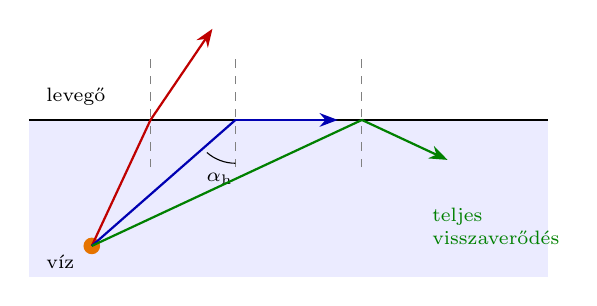
\begin{tikzpicture}[>=Stealth,font=\scriptsize]
  \fill[blue!8] (-2.2,-2.0) rectangle (4.4,0);
  \draw[thick] (-2.2,0) -- (4.4,0);
  \node[anchor=west] at (-2.1,0.3) {levegő};
  \node[anchor=west] at (-2.1,-1.8) {víz};
  \coordinate (S) at (-1.4,-1.6);
  \fill[orange!90!black] (S) circle (3pt);
  % 25 fok: kilép
  \draw[thick,red!75!black] (S) -- ++(0.746,1.6) coordinate (A);
  \draw[thick,red!75!black,->] (A) -- ++(55.8:1.4);
  \draw[dashed,gray] ($(A)+(0,-0.6)$) -- ($(A)+(0,0.8)$);
  % határszög
  \draw[thick,blue!70!black] (S) -- ++(1.825,1.6) coordinate (B);
  \draw[thick,blue!70!black,->] (B) -- ++(1.3,0);
  \draw[dashed,gray] ($(B)+(0,-0.6)$) -- ($(B)+(0,0.8)$);
  \draw ($(B)+(0,-0.55)$) arc (-90:-131.25:0.55);
  \node at ($(B)+(-0.2,-0.75)$) {$\alpha_\text{h}$};
  % 65 fok: teljes visszaverődés
  \draw[thick,green!50!black] (S) -- ++(3.431,1.6) coordinate (C);
  \draw[thick,green!50!black,->] (C) -- ++(-25:1.2);
  \draw[dashed,gray] ($(C)+(0,-0.6)$) -- ($(C)+(0,0.8)$);
  \node[green!50!black,anchor=west,align=left] at (2.8,-1.35) {teljes\\visszaverődés};
\end{tikzpicture}

\vspace{12pt}
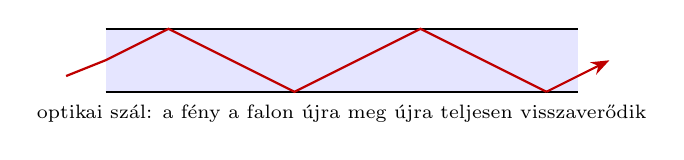
\begin{tikzpicture}[>=Stealth,font=\scriptsize]
  \fill[blue!10] (0,0) rectangle (6,0.8);
  \draw[thick] (0,0) -- (6,0); \draw[thick] (0,0.8) -- (6,0.8);
  \draw[thick,red!75!black] (-0.5,0.2) -- (0,0.4) -- (0.8,0.8) -- (2.4,0) -- (4.0,0.8)
     -- (5.6,0);
  \draw[thick,red!75!black,->] (5.6,0) -- (6.4,0.4);
  \node[below] at (3,-0.05) {optikai szál: a fény a falon újra meg újra teljesen visszaverődik};
\end{tikzpicture}

\vspace{12pt}
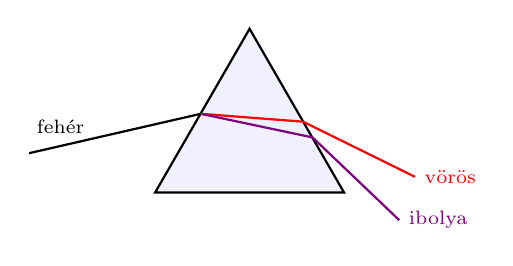
\begin{tikzpicture}[>=Stealth,font=\scriptsize]
  \draw[thick,fill=blue!6] (0,0) -- (2.4,0) -- (1.2,2.08) -- cycle;
  \draw[thick] (-1.6,0.5) -- (0.58,1.0);
  \node[above] at (-1.2,0.62) {fehér};
  \draw[thick,red] (0.58,1.0) -- (1.88,0.9) -- (3.3,0.2);
  \draw[thick,violet] (0.58,1.0) -- (2.0,0.7) -- (3.1,-0.35);
  \node[red,right] at (3.3,0.2) {vörös};
  \node[violet,right] at (3.1,-0.35) {ibolya};
\end{tikzpicture}
\end{minipage}

%====================================================================
\dia{3. Gömbtükrök és lencsék}

\begin{minipage}[t]{0.56\linewidth}\vspace{0pt}
\begin{itemize}
  \item \textbf{Gyűjtőlencse} (közepén vastagabb) és \textbf{homorú tükör}: a tengellyel
    párhuzamos sugarakat a \textbf{fókuszpontba} ($F$) gyűjti. Fókusztávolság: $f > 0$.
  \item \textbf{Szórólencse} (közepén vékonyabb) és \textbf{domború tükör}: a párhuzamos
    sugarakat úgy szórja szét, mintha $F$-ből jönnének. Ilyenkor $f < 0$.
  \item Gömbtükörnél $f = R/2$ ($R$ a görbületi sugár). \;
    \textbf{Dioptria:} $D = \dfrac1f$ ($f$ méterben), egysége $\tfrac1{\text{m}}$.
\end{itemize}
\begin{fontos}
\textbf{Nevezetes sugármenetek} (gyűjtőlencse):\\[2pt]
\textcolor{red!75!black}{\textbf{1.}} a tengellyel párhuzamos sugár $\to$ a túloldali $F$-en át;\\
\textcolor{orange!85!black}{\textbf{2.}} az optikai középponton átmenő sugár $\to$ irányváltozás nélkül;\\
\textcolor{violet}{\textbf{3.}} a fókuszponton átmenő sugár $\to$ a tengellyel párhuzamosan.\\[2pt]
Tükörnél ugyanígy, csak a sugarak visszaverődnek.
\end{fontos}
\begin{itemize}
  \item \textbf{Valódi kép:} a sugarak ténylegesen ott találkoznak, ernyőn felfogható.
    \textbf{Látszólagos kép:} csak a sugarak meghosszabbításai találkoznak, ernyőn nem
    fogható fel, csak belenézve látjuk (ilyen a sík tükör képe is).
\end{itemize}
\begin{pelda}
Kétszer domború üveglencse, $n = 1{,}5$, $R_1 = R_2 = 20$~cm:
$\tfrac1f = 0{,}5\cdot\bigl(\tfrac1{20} + \tfrac1{20}\bigr)~\tfrac1{\text{cm}}$ $\Rightarrow$
$f = 20$~cm, $D = 5$~dioptria. Egy $R = 40$~cm-es homorú tükörnek is $f = 20$~cm.
\end{pelda}
\end{minipage}\hfill
\begin{minipage}[t]{0.41\linewidth}\vspace{0pt}\centering
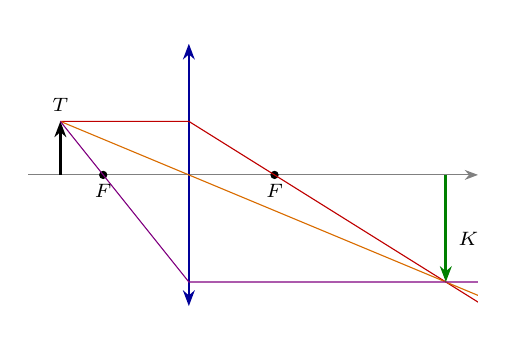
\begin{tikzpicture}[x=0.68cm,y=0.68cm,>=Stealth]
  \lenskep{1.6}{2.4}{1}{-3}{5.4}
  \node[font=\scriptsize] at (-2.4,1.3) {$T$};
  \node[font=\scriptsize,anchor=west] at (4.85,-1.2) {$K$};
\end{tikzpicture}\\
{\small gyűjtőlencse: valódi, fordított kép}

\vspace{6pt}
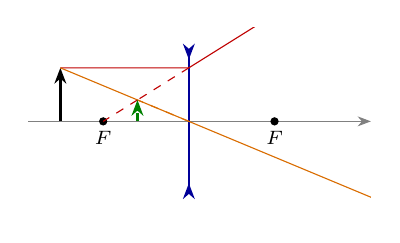
\begin{tikzpicture}[x=0.68cm,y=0.68cm,>=Stealth]
  \lenskep{-1.6}{2.4}{1}{-3}{3.4}
\end{tikzpicture}\\
{\small szórólencse: látszólagos, egyenes, kicsinyített kép}

\vspace{2pt}
\begin{fontos}[title=Lencsekészítő formula,fonttitle=\bfseries]
\[ \frac1f = (n-1)\left(\frac1{R_1} + \frac1{R_2}\right) \]
\small $n$: a lencse anyagának törésmutatója a környezethez képest (levegőben $n$,
vízben $n_\text{lencse}/n_\text{víz}$). Domború lap: $R > 0$, homorú lap: $R < 0$,
sík lap: $\tfrac1R = 0$.
\end{fontos}
\end{minipage}

%====================================================================
\dia{4. A leképezési törvény}

\begin{minipage}[t]{0.42\linewidth}\vspace{0pt}
\begin{fontos}
\[ \frac1f = \frac1t + \frac1k \qquad\qquad N = \frac{K}{T} = \frac{|k|}{t} \]
$t$: tárgytávolság, $k$: képtávolság, $T$, $K$: tárgy- és képnagyság.\\[2pt]
\textbf{Előjelek:} $k > 0$: valódi (fordított) kép; $k < 0$: látszólagos (egyenes) kép;
szórólencsénél és domború tükörnél $f < 0$.
\end{fontos}
Ugyanez a törvény érvényes lencsékre és gömbtükrökre is.
\begin{pelda}
Gyűjtőlencse, $f = 10$~cm.\\[2pt]
$t = 15$~cm: \quad $\dfrac1k = \dfrac1{10} - \dfrac1{15} = \dfrac1{30}$\\[2pt]
$\Rightarrow$ $k = 30$~cm, $N = 2$: valódi, fordított, nagyított.\\[4pt]
$t = 5$~cm: \quad $\dfrac1k = \dfrac1{10} - \dfrac15 = -\dfrac1{10}$\\[2pt]
$\Rightarrow$ $k = -10$~cm, $N = 2$: látszólagos, egyenes, nagyított
(a kép a tárggyal azonos oldalon van).
\end{pelda}
\end{minipage}\hfill
\begin{minipage}[t]{0.555\linewidth}\vspace{0pt}
\textbf{Gyűjtőlencse (és homorú tükör) képei:}\\[4pt]
\renewcommand{\arraystretch}{1.35}
\small\setlength{\tabcolsep}{4pt}
\begin{tabular}{|l|l|p{4.3cm}|p{2.6cm}|}
\hline
\textbf{tárgy} & \textbf{kép} & \textbf{jellege} & \textbf{példa} \\ \hline
$t > 2f$ & $f < k < 2f$ & valódi, fordított, kicsinyített & fényképezőgép, szem \\ \hline
$t = 2f$ & $k = 2f$ & valódi, fordított, $N = 1$ & \\ \hline
$f < t < 2f$ & $k > 2f$ & valódi, fordított, nagyított & vetítő \\ \hline
$t = f$ & nincs kép & a sugarak párhuzamosak & reflektor \\ \hline
$t < f$ & $k < 0$ & látszólagos, egyenes, nagyított & nagyító \\ \hline
\end{tabular}

\vspace{8pt}
\normalsize
\textbf{Szórólencse és domború tükör:} mindig látszólagos, egyenes, kicsinyített kép
(pl.\ a kereszteződésben lévő domború tükör nagy látószöget ad).

\vspace{6pt}
\textbf{Ökölszabály:} minél közelebb visszük a tárgyat a fókuszponthoz, annál távolabb és
annál nagyobb lesz a kép.
\end{minipage}

%====================================================================
\dia{5. A szem és az optikai eszközök}

\begin{minipage}[t]{0.58\linewidth}\vspace{0pt}
\begin{itemize}
  \item \textbf{A szem} gyűjtőlencse-rendszer (szaruhártya $+$ szemlencse): a retinán
    valódi, fordított, kicsinyített kép keletkezik. A képtávolság (a szem mérete) adott, ezért
    a szem a \textbf{fókusztávolságot} változtatja: a szemlencse domborúbb lesz
    (\textbf{alkalmazkodás}). Tiszta látás távolsága: $\approx 25$~cm.
  \item \textbf{Rövidlátás:} a távoli tárgy képe a retina \emph{előtt} keletkezik, a távoli
    tárgyak elmosódnak. Javítás: \textbf{szórólencse} (negatív dioptria).\\
    \textbf{Távollátás} (és időskori ,,öregszeműség''): a közeli tárgy képe a retina
    \emph{mögött} lenne. Javítás: \textbf{gyűjtőlencse}.
  \item \textbf{Nagyító:} gyűjtőlencse, a tárgy a fókuszon belül van.
    \textbf{Fényképezőgép:} $t > 2f$, a kép az érzékelőn; élesre állításkor a lencse és az
    érzékelő távolságát változtatjuk. \textbf{Vetítő:} $f < t < 2f$.
  \item \textbf{Mikroszkóp, csillagászati távcső:} két gyűjtőlencse. Az objektív valódi képét
    az okulárral, mint nagyítóval nézzük.
\end{itemize}
\begin{pelda}
Egy rövidlátó távolpontja $2$~m (ennél távolabb nem lát élesen). A szemüveg a végtelen
távoli tárgyról $2$~m-re lévő látszólagos képet készít:
$\dfrac1f = \dfrac1\infty + \dfrac1{-2~\text{m}}$ $\Rightarrow$ $f = -2$~m,
$D = -0{,}5$~dioptria (szórólencse).
\end{pelda}
\end{minipage}\hfill
\begin{minipage}[t]{0.38\linewidth}\vspace{0pt}\centering
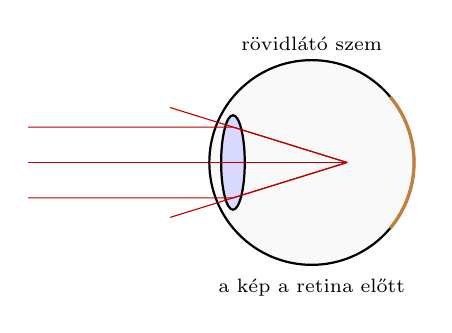
\begin{tikzpicture}[>=Stealth,font=\scriptsize]
  \draw[thick,fill=gray!5] (0,0) circle (1.3);
  \draw[very thick,brown] (40:1.3) arc (40:-40:1.3);
  \draw[thick,fill=blue!15] (-1.0,0) ellipse (0.15 and 0.6);
  \foreach \y in {0.45,0,-0.45} {
    \draw[red!75!black] (-3.6,\y) -- (-1.0,\y) -- (0.45,0);
    \draw[red!75!black] (0.45,0) -- ($(0.45,0)!1.55!(-1.0,\y)$);}
  \node[above] at (0,1.3) {rövidlátó szem};
  \node[below,align=center] at (0,-1.35) {a kép a retina előtt};
\end{tikzpicture}

\vspace{10pt}
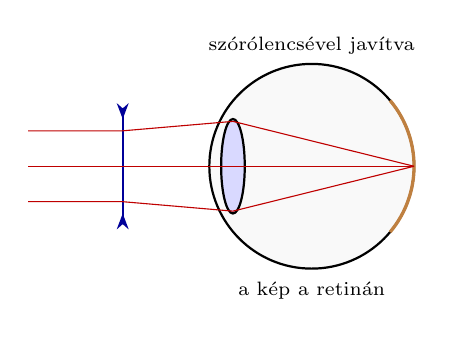
\begin{tikzpicture}[>=Stealth,font=\scriptsize]
  \draw[thick,fill=gray!5] (0,0) circle (1.3);
  \draw[very thick,brown] (40:1.3) arc (40:-40:1.3);
  \draw[thick,fill=blue!15] (-1.0,0) ellipse (0.15 and 0.6);
  \draw[{Stealth[length=2mm,reversed]}-{Stealth[length=2mm,reversed]},thick,blue!60!black] (-2.4,-0.8) -- (-2.4,0.8);
  \foreach \y/\z in {0.45/0.57,0/0,-0.45/-0.57} {
    \draw[red!75!black] (-3.6,\y) -- (-2.4,\y) -- (-1.0,\z) -- (1.3,0);}
  \node[above] at (0,1.3) {szórólencsével javítva};
  \node[below,align=center] at (0,-1.35) {a kép a retinán};
\end{tikzpicture}
\end{minipage}

%====================================================================
\dia{6. Összefoglalás}

\begin{minipage}[t]{0.48\linewidth}\vspace{0pt}
\begin{fontos}[title=Fénytörés,fonttitle=\bfseries]
\renewcommand{\arraystretch}{1.6}
\begin{tabular}{@{}ll@{}}
visszaverődés & $\alpha = \alpha'$ \\
törésmutató & $n = \dfrac{c}{c_\text{közeg}}$, \; $\lambda_\text{közeg} = \dfrac{\lambda_0}{n}$ \\
törési törvény & $\dfrac{\sin\alpha}{\sin\beta} = \dfrac{n_2}{n_1} = \dfrac{c_1}{c_2}$ \\
határszög & $\sin\alpha_\text{h} = \dfrac{n_2}{n_1}$ \; (csak ha $n_1 > n_2$) \\
színszóródás & ibolya törik a legjobban \\
\end{tabular}
\end{fontos}
\end{minipage}\hfill
\begin{minipage}[t]{0.49\linewidth}\vspace{0pt}
\begin{fontos}[title=Leképezés,fonttitle=\bfseries,colback=green!3,colframe=green!45!black]
\renewcommand{\arraystretch}{1.6}
\begin{tabular}{@{}ll@{}}
leképezési törvény & $\dfrac1f = \dfrac1t + \dfrac1k$ \\
nagyítás & $N = \dfrac{K}{T} = \dfrac{|k|}{t}$ \\
gömbtükör & $f = R/2$ \\
lencse & $\tfrac1f = (n-1)\bigl(\tfrac1{R_1} + \tfrac1{R_2}\bigr)$ \\
dioptria & $D = 1/f$ \; ($f$ méterben) \\
előjelek & $k < 0$: látszólagos; \; $f < 0$: szóró \\
\end{tabular}
\end{fontos}

\begin{fontos}[colback=yellow!8,colframe=orange!70!black,title=Házi feladat,fonttitle=\bfseries]
A feladatlap órán meg nem oldott feladatai, és egy szóbeli tétel elmondása (3--4 perc).
\end{fontos}
\end{minipage}

%====================================================================
\dia{7. Melléklet: képszerkesztés lencsékkel -- az összes eset}

{\small\jel{red!75!black} tengellyel párhuzamos sugár \quad
\jel{orange!85!black} optikai középponton átmenő sugár \quad
\jel{violet} fókuszon átmenő sugár \quad
\textcolor{green!50!black}{\textbf{$\uparrow$}} kép\\
szaggatott vonal: a sugarak meghosszabbítása, látszólagos kép}

\vspace{4pt}
\noindent
\cella{\Lkep{1.2}{3}{0.7}{-3.4}{3.2}}{\textbf{Gyűjtő, $t > 2f$:} valódi, fordított,
  kicsinyített; $f < k < 2f$ \\ (fényképezőgép, szem)}\hfill
\cella{\Lkep{1.2}{2.4}{0.7}{-2.9}{3.2}}{\textbf{Gyűjtő, $t = 2f$:} valódi, fordított,
  azonos méretű ($N = 1$); $k = 2f$}\hfill
\cella{\Lkep{1.2}{1.8}{0.7}{-2.9}{4.1}}{\textbf{Gyűjtő, $f < t < 2f$:} valódi, fordított,
  nagyított; $k > 2f$ \\ (vetítő)}

\vspace{8pt}
\noindent
\cella{\Lkep{1.2}{1.2}{0.7}{-2.9}{3.4}}{\textbf{Gyűjtő, $t = f$:} nincs kép, a kilépő
  sugarak párhuzamosak (a kép ,,a~végtelenben'' van)}\hfill
\cella{\Lkep{1.2}{0.7}{0.7}{-2.9}{2.9}}{\textbf{Gyűjtő, $t < f$:} látszólagos, egyenes,
  nagyított; $k < 0$, a tárgy oldalán \\ (nagyító)}\hfill
\cella{\Lkep{-1.2}{2.0}{0.7}{-2.9}{2.9}}{\textbf{Szóró, bármely $t$:} látszólagos, egyenes,
  kicsinyített; a kép $F$ és a lencse között \\ (rövidlátó szemüvege)}

%====================================================================
\dia{8. Melléklet: képszerkesztés gömbtükrökkel -- az összes eset}

{\small\jel{red!75!black} tengellyel párhuzamos sugár \quad
\jel{orange!85!black} a tükör közepébe érkező sugár (szimmetrikusan verődik vissza) \quad
\jel{violet} fókuszon átmenő sugár\\
$C$: görbületi középpont, $R = 2f$ \quad szaggatott vonal: a sugarak meghosszabbítása, látszólagos kép}

\vspace{4pt}
\noindent
\cella{\Tkep{1.2}{3}{0.7}{-3.4}{0.6}}{\textbf{Homorú, $t > 2f$:} valódi, fordított,
  kicsinyített; a kép $F$ és $C$ között}\hfill
\cella{\Tkep{1.2}{2.4}{0.7}{-3.0}{0.6}}{\textbf{Homorú, $t = 2f$:} valódi, fordított,
  azonos méretű; a kép $C$-ben}\hfill
\cella{\Tkep{1.2}{1.8}{0.7}{-4.1}{0.6}}{\textbf{Homorú, $f < t < 2f$:} valódi, fordított,
  nagyított; a kép $C$-n túl}

\vspace{8pt}
\noindent
\cella{\Tkep{1.2}{1.2}{0.7}{-3.2}{0.6}}{\textbf{Homorú, $t = f$:} nincs kép, a visszavert
  sugarak párhuzamosak \\ (reflektor, zseblámpa)}\hfill
\cella{\Tkep{1.2}{0.7}{0.7}{-2.9}{2.2}}{\textbf{Homorú, $t < f$:} látszólagos, egyenes,
  nagyított; a tükör mögött \\ (borotválkozótükör)}\hfill
\cella{\Tkep{-1.2}{2.0}{0.7}{-2.4}{2.8}}{\textbf{Domború, bármely $t$:} látszólagos, egyenes,
  kicsinyített; a tükör mögött \\ (közlekedési tükör)}

\vspace{6pt}
{\small A valódi kép a tükör \emph{előtt} keletkezik (ott fogható fel ernyőn), a látszólagos
a tükör \emph{mögött}.}

\end{document}
